\documentclass[11pt,oneside]{uhthesis}
%\documentclass[11pt,oneside]{report}
\usepackage{subfigure}
% \usepackage[linesnumbered,lined,titlenumbered,ruled]{algorithm2e}
\usepackage{amsmath}
\usepackage{amssymb}
\usepackage{amsbsy}
\usepackage{mathpazo}
\usepackage{float}
\usepackage{braket}
\setlength {\marginparwidth }{3cm}
\usepackage{todonotes}
\usepackage{bookmark}
\usepackage{soul}

\usepackage[spanish]{babel}
\usepackage{graphicx}
\usepackage{icomma}
\decimalpoint
\usepackage{listings}
\usepackage{color}
\usepackage{booktabs}
\usepackage{multirow}
\usepackage{ragged2e}

\floatstyle{ruled}
\restylefloat{table}
\usepackage{listings}
\usepackage{color}

\usepackage{algorithm}
\usepackage{algpseudocode}

\definecolor{dkgreen}{rgb}{0,0.6,0}
\definecolor{gray}{rgb}{0.2,0,0}
\definecolor{mauve}{rgb}{0.58,0,0.82}

\lstset{language=Lisp,
	aboveskip=10mm,
	belowskip=10mm,
	showstringspaces=false,
	columns=flexible,
	basicstyle={\small\ttfamily},
	keywordstyle=\color{blue},
	commentstyle=\color{dkgreen},
	stringstyle=\color{mauve},
	breaklines=true,
	breakatwhitespace=true,
	tabsize=3,
	numbers=left, numberstyle=\tiny, stepnumber=1,firstnumber=1,
	numbersep=5pt
}

\renewcommand{\tablename}{Tabla}
\title{Análisis Computacional de Coros de \emph{Eleutherodactylus eileenae} (Dunn, 1926): Inferencia de Redes desde Señales Bioacústicas}
\author{Daniel Machado Pérez}
\advisor{\\\vspace{0.25cm}Dr. Roberto Mulet Genicio\\\vspace{0.25cm}Dr. Milton García Borroto}
\degree{Licenciado en Ciencia de la Computación}
\faculty{Facultad de Matemática y Computación}
\date{La Habana, \\mayo 2025\\\vspace{0.25cm}\href{https://github.com/DanielMPMatCom/Thesis.git}{github.com/DanielMPMatCom/Thesis.git}}
\logo{Graphics/uhlogo}

\renewcommand{\vec}[1]{\boldsymbol{#1}}
\newcommand{\diff}[1]{\ensuremath{\mathrm{d}#1}}

\begin{document}
\selectlanguage{spanish}

%\frontmatter
\maketitle

\begin{dedication}
	\textit{
		"La utopía está en el horizonte\\
		Camino dos pasos y se aleja dos pasos.\\
		Camino diez y el horizonte se corre diez pasos más allá.\\
		Entonces, ¿para qué sirve la utopía?\\
		Para eso, sirve para caminar."\\}
		\begin{flushright}
			\textbf{Fernando Birri}
		\end{flushright}
		\vspace{1cm}
\end{dedication}
\chapter*{Agradecimientos}\label{chapter:agradecimientos}


El autor agradece al Dr. Roberto Alonso 
Bosch y la M.Sc. Mariam Curbelo Cruz por facilitar los datos de 
campo, 
compartir su amplia experiencia sobre el 
comportamiento de \emph{Eleutherodactylus 
eileenae}, orientar la revisión de la 
literatura especializada y la revisión del manuscrito.

Por supuesto, también extiende su profundo agradecimiento a los 
tutores Dr. Roberto Mulet y Dr. Milton
García, por su paciencia, dedicación, experiencia y por el regalo 
de una formación que abarca mucho más que el ámbito científico.  
\begin{abstract}
    El análisis computacional de coros animales representa un 
desafío en ecoacústica, particularmente en ambientes con 
superposición de señales y ruido. Esta investigación 
desarrolló un flujo automatizado para procesar grabaciones 
de \emph{Eleutherodactylus eileenae}, una rana endémica de 
Cuba cuyos machos forman coros nocturnos para atraer a las hembras. 
Se aplicó un filtrado espectral basado en percentiles 
para atenuar interferencias de banda ancha y puntuales. A continuación, 
nueve pistas de audio se sincronizaron mediante correlación cruzada. 
Se implementaron dos algoritmos heurísticos para detectar y asignar 
cantos a micrófonos: uno basado en hipótesis de energías relativas a los audios 
y otro mediante \emph{clustering} espectro-temporal, este último 
mostrando mayor precisión en condiciones de baja actividad. Las series 
temporales resultantes se modelaron como una red de espines usando 
el modelo de Ising, cuyos parámetros \(J_{ij}\) se inferieron por 
máxima verosimilitud. Aunque se identificaron acoplamientos significativos, 
el modelo independiente superó al de Ising en la predicción de patrones, 
sugiriendo interacciones débiles o limitaciones en la formulación estándar 
del modelo. El trabajo demuestra que enfoques heurísticos reproducibles 
permiten reconstruir dinámicas colectivas en coros y propone mejoras 
metodológicas para futuros estudios.
\end{abstract}

\begin{enabstract}
The computational analysis of animal choruses poses a significant 
challenge in ecoacoustics, particularly in environments with 
signal overlap and noise. This study developed an automated pipeline 
to process recordings of \emph{Eleutherodactylus eileenae}, a frog 
endemic to Cuba whose males form nocturnal choruses to attract females. 
First, spectral filtering based on amplitude percentiles was applied 
to attenuate both broadband and transient interference. Then, nine audio 
tracks were synchronized via cross-correlation. Two heuristic algorithms 
were implemented to detect and assign calls to microphones: one based 
on hypotheses of relative energy in the recordings and another using 
spectro-temporal clustering, the latter demonstrating higher accuracy 
under low activity conditions. The resulting time series were modeled 
as a spin network using the Ising model, with interaction parameters 
\(J_{ij}\) inferred via maximum likelihood. Although significant 
couplings were identified, an independent model outperformed the 
Ising model in predicting call patterns, suggesting either weak 
interactions or limitations in the standard model formulation. This 
work demonstrates that reproducible heuristic approaches can reconstruct 
collective dynamics in animal choruses and proposes methodological 
improvements for future studies.
\end{enabstract}
\tableofcontents
\listoffigures


%\mainmatter
	
%===================================================================================
% Chapter: Introduction
%===================================================================================
\chapter*{Introducción}\label{chapter:introduction}
\addcontentsline{toc}{chapter}{Introducción}
%===================================================================================

\qquad 


Las técnicas de monitorización acústica automatizada se han 
convertido en una herramienta esencial para el estudio de 
comunidades de animales en su medio natural. En particular, el 
análisis del canto de los anuros ofrece información valiosa 
sobre sus estrategias de apareamiento, la dinámica de sus 
poblaciones y la salud de los ecosistemas en los que habitan \cite{blumstein2011acoustic}. 
La rana cubana \emph{Eleutherodactylus eileenae} (Dunn, 1929), 
endémica de Cuba, constituye un modelo idóneo para investigar 
estos procesos, pues sus machos forman coros nocturnos cuyos 
patrones de interacción pueden reflejar aspectos tanto 
ecológicos como de comportamiento social \cite{alonso2001patrones}.


\emph{E. eileenae}, conocido comúnmente como “Colín”, es una especie perteneciente 
a la familia \emph{Eleutherodactylidae}. Su distribución abarca desde la península 
de Guanahacabibes, en Pinar del Río, hasta la Sierra de Najasa, en Camagüey, ocupando 
diversos hábitats como bosques semideciduos, pinares y cafetales, hasta altitudes de 
aproximadamente 900 metros sobre el nivel del mar \cite{alonso2001patrones,schwartz1958new,estrada1994herpetofauna}. Durante 
el día, estos anuros se refugian en oquedades de rocas, troncos, hojarasca y 
bromelias; al anochecer, los machos ascienden a ramas y hojas, hasta alturas de 3 
metros, para emitir sus vocalizaciones.

El canto característico de \emph{E.\,eileenae} consta de dos notas diferenciadas: 
una primera “Co”, breve y de frecuencia menor, seguida de una segunda “Lin”, más 
prolongada y de frecuencia ligeramente superior. Esta estructura ha motivado el uso 
del término “Colín” para referirse tanto a cada canto individual como, 
coloquialmente, a la especie misma. Estas llamadas desempeñan un papel crucial en la 
comunicación intraespecífica, mediando aspectos relacionados con el estado 
fisiológico y la competencia territorial \cite{alonso2001patrones}. Además, se ha observado que los machos 
forman agrupaciones o “coros”, sincronizando sus cantos para aumentar la eficacia en 
la atracción de hembras y reducir el riesgo de depredación.

La presente investigación desarrolla un flujo computacional automatizado para 
procesar grabaciones de los cantos de los Colines y, a partir de él, comenzar a analizar 
 las interacciones acústicas asociadas a estos coros. 
El objetivo es comprender las 
estrategias de comunicación que emplea \emph{E.\,eileenae} en su entorno natural.
En la Figura \ref{fig:colin} se muestra un ejemplar de esta especie, y en la
Guía sonora de los anfibios de Cuba 
\footnote{Grabación disponible en: \url{https://www.fonozoo.com/fnz_detalles_registro_amphibia.php?id=97953&tipo_registro=1}}
se puede encontrar una breve grabación de su canto y otros datos relevantes.\\

\begin{figure}[h!]
    \centering
    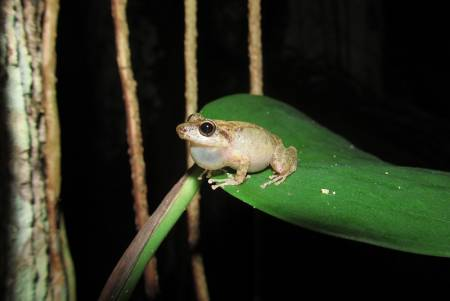
\includegraphics[width=\columnwidth]{Graphics/colin.jpg}
    \caption{Ejemplar de \emph{Eleutherodactylus eileenae}.}
    \label{fig:colin}
\end{figure}


\section{Motivación y justificación}
\label{sec:motivacion_justificacion}

La ecoacústica ha evolucionado desde la grabación pasiva hasta flujos computacionales 
que automatizan la detección de llamadas en ambientes ruidosos 
\cite{acevedo2009automated,blumstein2011acoustic}. Sin embargo, en Cuba pocos estudios 
han integrado estas técnicas con modelos de interacción y causalidad.

El análisis manual de grabaciones de campo resulta lento, 
costoso y propenso a errores humanos, lo que limita la escala y 
reproducibilidad de los estudios bioacústicos. En trabajos 
previos sobre \emph{E.\,eileenae}, los investigadores 
describieron manualmente las etapas de vocalización y 
realizaron muestreos puntuales de la actividad acústica y 
trófica de los machos en la Sierra del Rosario \cite{alonso2001patrones}. 
Sin embargo, no se abordó la sincronización automática de 
múltiples micrófonos ni la clasificación sistemática de cada 
llamado, pasos indispensables para escalar el análisis a largas 
series temporales y diferentes localidades.

Además, los coros de machos implican interacciones acústicas 
cuya dinámica no se comprende completamente: ¿cómo influyen la 
densidad de individuos, la configuración espacial de los 
micrófonos y el ruido ambiental en la estructura del coro? 
¿Qué reglas simples de interacción subyacen en la sincronización 
de los “Colines”? En este contexto, un enfoque computacional reproducible
y basado en algoritmos heurísticos permitiría procesar de 
manera eficiente decenas de horas de grabaciones, discriminando 
eventos de interés (cantos de Colines) de otros sonidos 
(otra fauna, viento, tráfico) y garantizando resultados 
comparables entre campañas de muestreo.

Los resultados de la presente tesis constituyen un primer paso hacia 
el desarrollo de un 
flujo completo que abarque, desde la adquisición y sincronización 
de señales, hasta la clasificación automática de cantos y el 
modelado de interacciones acústicas, a fin de superar las 
limitaciones de los métodos manuales y aportar herramientas 
robustas para la ecoacústica de anfibios en Cuba y regiones 
semejantes.

\section{Formulación del problema}
\label{sec:formulacion_problema}

El presente trabajo se ocupa del procesamiento automático de un 
conjunto de grabaciones registradas en la Reserva de 
la Biosfera “Sierra del Rosario” con el objetivo de 
caracterizar los cantos de machos de 
\emph{Eleutherodactylus eileenae} y reconstruir la dinámica de 
sus coros. Estas grabaciones, realizadas con nueve micrófonos 
omnidireccionales dispuestos en un área de aproximadamente 20 m 
de radio, abarcan ciclos de 58 minutos de registro seguidos de 
2 minutos de descarga, durante tres noches consecutivas entre 
las 18:00 y las 06:00 horas. El entorno de captura se ve 
afectado por ruido de lluvia, viento, tráfico y la superposición 
de cantos de varios individuos, lo que plantea retos importantes 
tanto en la sincronización de señales como en la discriminación 
de los eventos acústicos relevantes frente a emisiones no 
deseadas. En la Figura \ref{fig:map} se muestra la distribución geográfica de los micrófonos en el área de estudio.

\begin{figure}[h!]
    \centering
    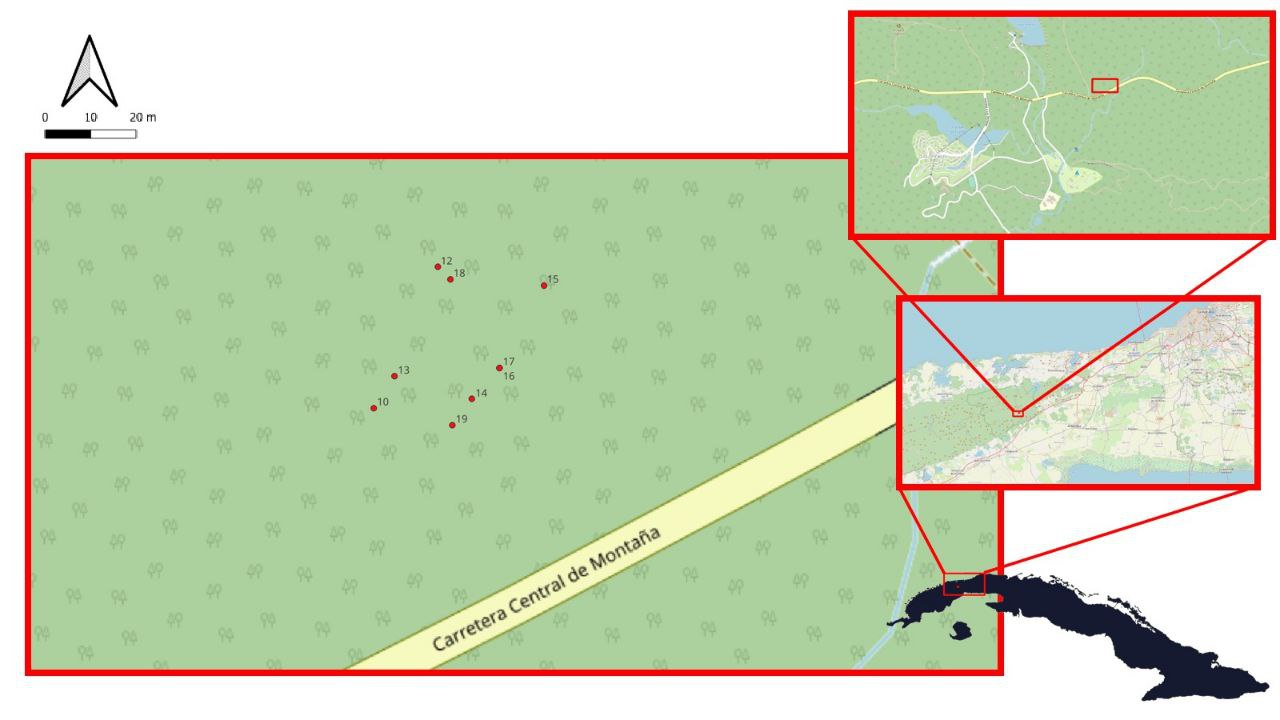
\includegraphics[width=\columnwidth]{Graphics/mic_map.jpg}
    \caption{Distribución Geográfica de los Micrófonos.}
    \label{fig:map}
\end{figure}

En este ámbito, el problema central consiste en el diseño de 
un flujo heurístico 
capaz de sincronizar con precisión las nueve pistas de audio, 
detectar de manera fiable los instantes de emisión de cada 
canto (“Colín”) y asignar cada evento al micrófono (y por tanto 
al individuo) correspondiente; a partir de ello, se extraen 
parámetros temporales y espectrales de cada llamado para 
generar un registro estructurado que sirve de base a la 
inferencia de una red de interacción inspirada en el modelo de 
Ising \cite{ising1925beitrag}. Se espera que la sincronización 
automática alcance una resolución temporal tal que permita 
distinguir llamadas superpuestas de machos vecinos, y que la 
combinación de criterios de proximidad y similitud espectral 
garantice una alta exactitud en la etiqueta de cada canto, 
validada mediante muestreo manual. Finalmente, las secuencias 
temporales resultantes se emplean para estimar los parámetros 
de interacción \(J_{ij}\), de modo que el modelo reproduzca 
con fidelidad las correlaciones de co-emisión observadas en el 
coro.  


La complejidad del problema reside en la superposición de 
señales y en la variabilidad del nivel de ruido ambiental, lo 
cual exige emplear técnicas robustas de filtrado. 
Este trabajo opta por heurísticas 
de intensidad relativa y correlación espectral para asignar cada “Colín” al micrófono y 
al individuo correspondiente, garantizando 
la reproducibilidad de los resultados y la comparabilidad con 
futuros estudios bioacústicos. Este estudio es el primero en 
Cuba en aplicar el modelo de Ising para describir 
interacciones acústicas en coros de anuros, siguiendo 
aproximaciones similares en redes 
neuronales y colonias de insectos \cite{schneidman2006weak,mora2011biological,bialek2012biophysics,reyes2019transmission,ising1925beitrag}.

\section{Hipótesis}
\label{sec:hipotesis}

Se plantea como hipótesis principal que un flujo computacional 
basado en algoritmos heurísticos para la sincronización, 
detección y clasificación de cantos de Colines podrá reproducir con un alto 
grado de fidelidad las secuencias de emisión de cada individuo 
y, a partir de ellas, inferir las interacciones acústicas 
subyacentes a la formación de coros. 


Esto fundamenta la 
viabilidad de un enfoque computacional replicable y escalable 
que, aplicado a los cantos de Colines, aporte 
nuevas perspectivas cuantitativas sobre la dinámica de los coros 
y sirva como base para futuros estudios comparativos en 
ecoacústica.  


\section{Objetivos}
\label{sec:objetivos}

El objetivo general de esta tesis es desarrollar y 
validar un flujo heurístico que, mediante la detección y 
clasificación de los cantos de \emph{E.\,eileenae}, permita 
reconstruir la dinámica de sus coros y cuantificar su 
sincronización y causalidad.
Para ello se plantean los siguientes objetivos específicos:

\begin{enumerate}
  \item \textbf{Construir un \emph{dataset} limpio y sincronizado:}  
    \begin{itemize}
      \item Sincronizar las nueve pistas de audio utilizando referencias comunes (picos de energía) y correlación cruzada.  \cite{costa2021comparing}
      \item Eliminar ruidos de fondo (lluvia, viento, tráfico) e interferencias no deseadas.
    \end{itemize}
  \item \textbf{Detectar y asignar cada canto a su emisor:}  
    \begin{itemize}
      \item Desarrollar heurísticas de proximidad basadas en la intensidad relativa en cada micrófono.  
      \item Validar la asignación mediante muestreo manual de segmentos y cálculo de exactitud.
      \item Evaluar la consistencia de los algoritmos de detección y asignación.
      \item Comparar el rendimiento de los algoritmos diseñados.
    \end{itemize}
  \item \textbf{Inferir un modelo de interacciones acústicas:}  
    \begin{itemize}
      \item Formular la red de interacciones como un modelo de Ising con parámetros \(J_{ij}\) que cuantifiquen la co-emisión.  
      \item Estimar los \(J_{ij}\) mediante el Principio de Máxima Verosimilitud \cite{fisher1912maximum} y algoritmos de descenso por gradiente.
      \item Evaluar la idoneidad del modelo de Ising mediante una comparación con el modelo Independiente en cuanto a su capacidad para predecir los patrones de cantos.
    \end{itemize}
\end{enumerate}


\section{Propuesta de solución}
\label{sec:propuesta_solucion}

Para dar respuesta al problema planteado, se propone un 
flujo de trabajo modular que integre cuatro etapas principales: 
sincronización, filtrado, asignación de 
emisores y modelado de interacciones. En primer lugar, la 
sincronización de las nueve pistas de audio se realiza 
mediante la aplicación de correlación cruzada sobre los histogramas
de distribución de distancias temporales entre los picos de energía de los audios 
y un punto de referencia. A continuación, se 
aplica un filtro que consiste en una poda espectral
basada en el percentil 99.9 de la amplitud por frecuencia.
Con ello se busca atenuar 
ruido de baja (viento, tráfico) y alta frecuencia (insectos).  

En la tercera fase se asigna cada 
llamado al micrófono más adecuado mediante heurísticas de 
intensidad relativa. 
Finalmente, la información temporal y espectral extraída de cada 
evento sirve para construir un grafo de interacciones, 
modelado con un enfoque de máxima verosimilitud en un sistema 
análogo al modelo de Ising. El ajuste de los 
parámetros \(J_{ij}\) se lleva a cabo mediante un algoritmo de 
descenso por gradiente.  

Este flujo, además de automatizar completamente la extracción de 
datos, permite validar la hipótesis mediante 
métricas objetivas de precisión y reproducibilidad, y ofrece 
una herramienta extensible a otros sistemas de ecoacústica con 
configuraciones similares.  


\section{Estructura del Documento}
\label{sec:estructura_documento}

Para explicar la solución propuesta y el flujo de trabajo, 
se diseñó la siguiente estructura del presente documento. 
En el Capítulo 1 se revisan los antecedentes y actualidad en cuanto a 
detección y 
clasificación de llamadas bioacústicas, con especial énfasis 
en métodos de sincronización y filtrado de señales. 
El Capítulo 2 detalla la metodología empleada: adquisición y 
preprocesamiento de las grabaciones, tanto el diseño de 
algoritmos heurísticos 
para la detección de los “Colines” como la asignación de cada 
canto a su emisor, y la formulación del modelo de interacciones 
basado en Ising con inferencia por máxima verosimilitud y 
descenso por gradiente. En el Capítulo 3 se presentan los 
resultados: evaluación de la precisión de 
sincronización, rendimiento de los detectores de canto, 
exactitud de la asignación micrófono-Colín y análisis de las 
interacciones inferidas \(\{J_{ij}\}\). Además en las 
Conclusiones se discuten las aportaciones principales, las 
implicaciones ecológicas y computacionales y las limitaciones 
del estudio.
Finalmente, en las Recomendaciones se presentarán sugerencias 
generales basadas en los resultados, destinadas a 
orientar mejoras metodológicas, proponer nuevas líneas de 
investigación y facilitar la aplicación práctica del enfoque 
desarrollado en estudios futuros.  

% -----------------------------------------------------------------------



% La rana \emph{Eleutherodactylus eileenae} (Dunn, 1929) es una especie 
% de la familia \emph{Eleutherodactylidae}, endémica de Cuba. 
% Se distribuye desde la península de Guanahacabibes, Pinar del Río, 
% hasta la Sierra de Najasa, en la provincia de Camagüey. 
% Ocupa hábitats como bosques semideciduos, pinares y cafetales
% en altitudes de hasta 900 metros sobre el nivel del mar. 
% Durante el día permanece oculta en
% oquedades de rocas y troncos, y entre la hojarasca y bromelias.
% Durante la noche los machos ascienden 
% para vocalizar en ramas y hojas de hasta 3 m de altura. \cite{alonso2001patrones}
% En la Figura \ref{fig:colin} se muestra un ejemplar de esta especie, y en la
% Guía sonora de los anfibios de Cuba 
% \footnote{Grabación disponible en: \url{https://www.fonozoo.com/fnz_detalles_registro_amphibia.php?id=97953&tipo_registro=1}}
% se puede encontrar una breve grabación de su canto y otros datos relevantes.\\

% \begin{figure}[h!]
%     \centering
%     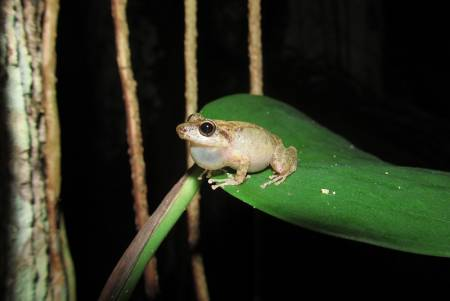
\includegraphics[width=\columnwidth]{Graphics/colin.jpg}
%     \caption{Ejemplar de \emph{Eleutherodactylus eileenae}.}
%     \label{fig:colin}
% \end{figure}


% El canto de \emph{E.\,eileenae} consta de dos notas 
% diferenciadas: una primera “Co” breve y de frecuencia menor, 
% seguida de “Lin” más prolongada y de frecuencia ligeramente 
% superior, nombradas de esta forma para imitar el sonido producido. 
% Por tal motivo y por simplicidad se procederá a nombrar “Colín” a cada uno de los cantos 
% y también se utilizará como nombre coloquial de la especie. 
% Estas llamadas median parámetros bioacústicos 
% vinculados al estado fisiológico y a la competencia territorial. 
% Además, se ha observado que los machos forman agrupaciones 
% (“coros”), sincronizando pulsos y modulaciones para incrementar 
% la eficacia de atracción de hembras y reducir el riesgo de 
% depredación. La presente investigación se centrará en el estudio de dichos
% coros y los cantos con fines de apareamiento de los Colines.



% \section{Características del \emph{dataset} de grabaciones}

% El canto de \emph{E.\,eileenae} se produce en la noche,
% cuando los machos se agrupan para vocalizar, 
% con picos de actividad en los meses calurosos y lluviosos del año y 
% en las horas de la tardenoche y la madrugada.
% Con el objetivo de adquirir datos para los estudios de la especie,
% el grupo de investigación dirigido por el Dr. Roberto Alonso, de la Facultad de Biología de la Universidad de La Habana,
% realizó un conjunto de grabaciones de campo en la zona de la 
% Reserva de la Biosfera “Sierra del Rosario”. Después de identificar ciertos
% individuos y los sitios donde usualmente se ubicaban para emitir sus cantos, se colocaron
% 9 micrófonos (cada uno aproximadamente a 1 metro de distancia de su Colín más cercano)
% cuya activación remota permitió el registro de la información acústica del coro en cuestión.
% Todos los dispositivos eran del mismo modelo, unidireccionales, y eran activados simultáneamente para comenzar a grabar
% 58 minutos consecutivos, utilizar 2 minutos para guardar los datos adquiridos y luego volver a comenzar a grabar.
% Esto se hizo durante 3 noches, en los períodos comprendidos entre las 18:00 horas y las 6:00 horas del día siguiente, entre los días
% 20 y 23 de octubre de 2023. En la Figura \ref{fig:map} se muestra la distribución geográfica de los micrófonos en el área de estudio.
% Como se puede apreciar, los micrófonos fueron colocados en un área con un radio de aproximadamente 20 metros.\\

% \begin{figure}[h!]
%     \centering
%     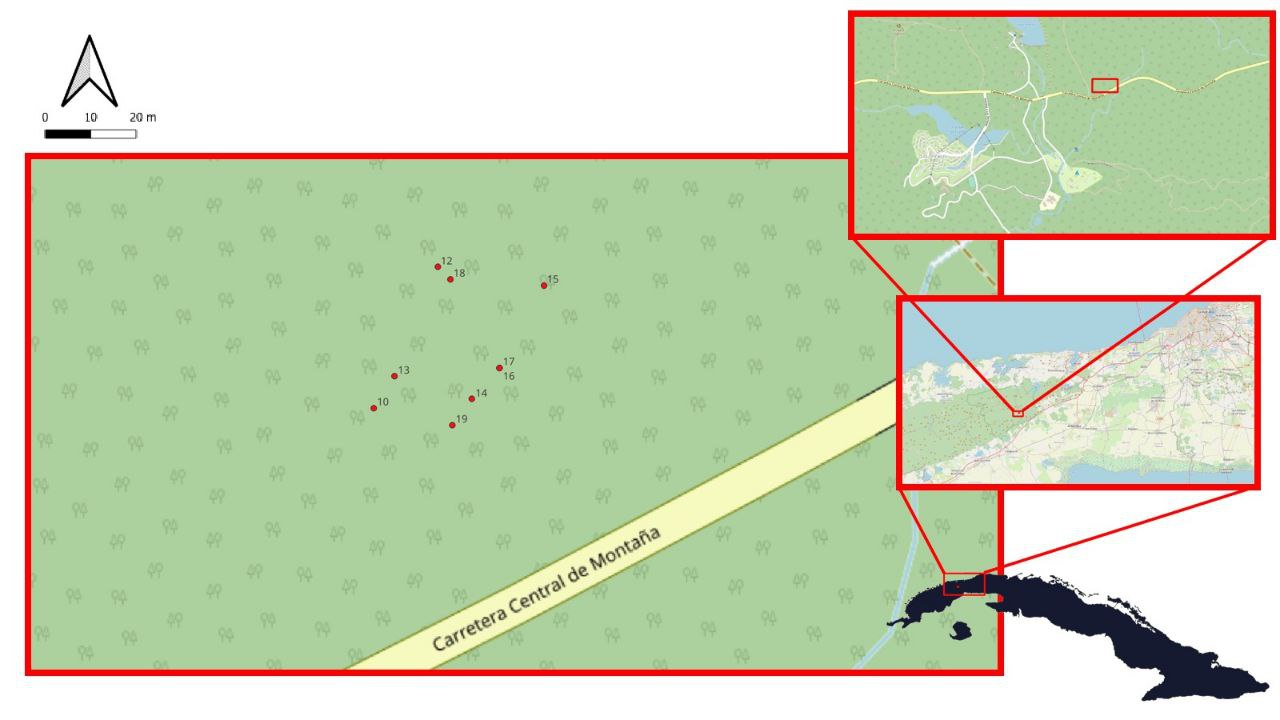
\includegraphics[width=\columnwidth]{Graphics/mic_map.jpg}
%     \caption{Distribución Geográfica de los Micrófonos.}
%     \label{fig:map}
% \end{figure}

% Debido a que los micrófonos son omnidireccionales y están situados 
% relativamente cercanos entre sí, en cada uno se registran no solamente
% los cantos del individuo de Colín más cercano, sino también cantos de especímenes
% cercanos, sonidos del ambiente natural de la zona, e incluso ruidos de 
% agentes artificales como autos pasando por una carretera cercana.



% \section{Motivaciones de la investigación}

% Como parte de los estudios sobre la ecología de esta especie de anuros
% se quiere profundizar en lo que se conoce sobre las características de sus cantos,
% de sus métodos de comunicación y su comportamiento social. Además se quiere 
% saber si realmente se organizan en coros, y si ese fuera el caso, analizar la
% estructura de dichos coros, la posible existencia de un líder o protagonista,
% o de manera general estudiar las interacciones en el sistema formado por los Colines
% machos mientras cantan para atraer a las hembras.\\

% Hasta el momento, el trabajo para procesar los audios recopilados se realizaba de forma manual
% con \emph{softwares} no automáticos. La identificación manual de cada llamado (etiquetado por 
% individuo, hora y localización) resulta extremadamente lenta, 
% sujeta a errores humanos y poco reproducible. Dichas razones,
% sumadas a la búsqueda de avances más eficientes y rigurosos, motivaron el tratamiento
% del problema desde un enfoque computacional, para automatizar los procesos
% y poder modelar matemáticamente el sistema de interacción entre los Colines.\\ 


% \section{Problema científico}

% El problema planteado consiste en, dado un \emph{dataset} de grabaciones
% de campo de un coro de Colines hechas con 9 micrófonos omnidireccionales,
% procesar los datos para obtener la información de los cantos de cada uno de 
% los individuos implicados (momento del canto, frecuencia, energía) para
% analizar la estructura de dicho coro. \\

% Que los dispositivos de sean omnidireccionales plantea la dificultad de
% que en una misma grabación se registra la información de sonidos que no interesan,
% como otros animales, autos e incluso Colines que no son los más cercanos al aparato.
% Por lo tranto surge la necesidad de diseñar un proceso para discriminar correctamente
% estos datos, y obtener una asigación Micrófono-Colín. Además es evidente que se impone
% encontrar una forma de eliminar el ruido y “limpiar” los audios. 
% También se debe verificar la correcta sincronización de las grabaciones,
% pues a pesar de la activación remota y simultánea, el posible error de \emph{hardware}
% podría comprometer la precisión de los resultados.\\

% Convendría modelar matemáticamente el sistema
% para cuantificar las interacciones entre los especímenes y llevar a cabo un estudio
% de causalidad. Para ello se propone la utilización de un recurso clásico
% de la Física Estadística, el Modelo de Ising. \cite{chau2017inverse}

% \section{Objetivos de la tesis}

% El objetivo principal de esta tesis es diseñar, implementar y validar un flujo computacional automatizado para la detección, clasificación y análisis de los cantos de apareamiento de \emph{Eleutherodactylus eileenae}, con el fin de reconstruir la estructura de sus coros y modelar las interacciones acústicas entre individuos mediante el enfoque del modelo de Ising.
% Para ello se plantean los siguientes objetivos específicos:

% \begin{enumerate}
%   \item Construir un \emph{dataset} limpio de grabaciones que permita extraer estadísticas fiables y facilitar la interpretación de resultados.
%   \item Desarrollar un método de sincronización automática de las señales grabadas por los nueve micrófonos para asegurar la consistencia temporal del \emph{dataset}.
%   \item Implementar técnicas de eliminación de ruido de fondo y filtrado de eventos no deseados (otros animales, vehículos, artefactos ambientales).
%   \item Diseñar y comparar algoritmos para la obtención de las secuencias de cantos de cada Colín.
%   \item Validar la consistencia, precisión y reproducibilidad de los métodos propuestos.
%   \item Modelar matemáticamente la red de interacciones acústicas entre individuos utilizando el modelo de Ising:
%     \begin{itemize}
%       \item Formulación del problema como Principio de Máxima Verosimilitud.
%       \item Implementación de algoritmos de Descenso por Gradiente para la inferencia de los parámetros \(J_{ij}\) (interacción entre el individuo $i$ y $j$).
%     \end{itemize}
%   \item Analizar la idoneidad del modelo de Ising para describir la causalidad en los coros, comparando las interacciones inferidas con comportamientos observados.
%   \item Interpretar los resultados y extraer conclusiones ecológicas y computacionales que permitan proponer recomendaciones para estudios bioacústicos futuros.
% \end{enumerate}

% Para abordar estos objetivos, la tesis se organiza en los siguientes capítulos:
% \begin{description}
%   \item[Capítulo 1:] \emph{Detección de individuos a partir de señales de audio}. Revisión del estado del arte en detección y clasificación de llamadas bioacústicas.
%   \item[Capítulo 2:] \emph{Métodos y metodologías}. Representación de audio como \emph{mel}-espectrogramas, sincronización, eliminación de ruido, diseño de algoritmos de identificación y discriminación de Colines, y formulación del modelo de Ising con su inferencia mediante máxima verosimilitud y descenso por gradiente.
%   \item[Capítulo 3:] \emph{Resultados e interpretación}. Evaluación de la sincronización automática, obtención de secuencias de cantos, hipótesis de comportamiento espectral, comparación de algoritmos, pruebas de consistencia y precisión, y análisis de las interacciones inferidas \(\{J_{ij}\}\) en el modelo de Ising.
%   \item[Conclusiones y Recomendaciones:] Síntesis de hallazgos, discusión de implicaciones ecológicas y computacionales, limitaciones del estudio y propuestas de trabajo futuro.
% \end{description}





% % \section*{Contexto histórico y social}
% % En las últimas décadas, el análisis automatizado de datos biológicos ha revolucionado campos tan diversos como la ecoacústica y los estudios de comportamiento colectivo. En particular, los avances en aprendizaje automático han permitido procesar grandes volúmenes de grabaciones de campo para monitorear especies silvestres de manera más precisa y reproducible :contentReference[oaicite:0]{index=0}. Paralelamente, la Física Estadística ha contribuido al entendimiento de sistemas complejos mediante modelos de interacción par a par, como el modelo de Ising, aplicado originariamente a redes de espines y recientemente extendido a inferencia de redes biológicas :contentReference[oaicite:1]{index=1}.  

% % \section*{Antecedentes del problema científico}
% % En Cuba, los estudios sobre comportamiento colectivo se han centrado tradicionalmente en sistemas como colonias de hormigas, demostrando cómo interacciones locales generan patrones globales de organización sin control centralizado :contentReference[oaicite:2]{index=2}. En el ámbito de los anfibios, la comunicación acústica ha servido como modelo para entender la señalización social y la toma de decisiones del sistema nervioso :contentReference[oaicite:3]{index=3}. Sin embargo, la mayoría de los análisis de cantos de ranas se realiza aún de forma manual, lo que limita la escala y reproducibilidad de los estudios :contentReference[oaicite:4]{index=4}.

% % \section*{Breve presentación de la problemática}
% % La rana cubana \emph{Eleutherodactylus eileenae} (Dunn, 1929) es un anuro endémico que forma coros de machos durante la noche para atraer hembras. Cada canto, denominado “Colín”, consta de dos notas diferenciadas (“Co” y “Lin”) que varían en frecuencia y duración :contentReference[oaicite:5]{index=5}. Para estudiar la estructura de estos coros y las interacciones acústicas entre individuos, se dispusieron redes de micrófonos que registraron cientos de horas de audio en ambientes ruidosos, lo que plantea retos de sincronización, filtrado de ruido y asignación automática de cada evento acústico a su emisor :contentReference[oaicite:6]{index=6}.

% % \section*{Actualidad y novedad científica}
% % Hoy día, la integración de sensores pasivos con algoritmos de inteligencia artificial permite extraer patrones bioacústicos a escala inédita :contentReference[oaicite:7]{index=7}. No obstante, aplicar modelos de inferencia estadística, como el modelo de Ising, para cuantificar las interacciones en un coro de ranas nocturnas constituye una aproximación novedosa que une ecoacústica, teoría de redes y computación biomédica.  

% % \section*{Importancia teórica y práctica}
% % Teóricamente, el estudio contribuirá a validar el modelo de Ising en sistemas biológicos reales, más allá de ensayos in silico :contentReference[oaicite:8]{index=8}. Prácticamente, facilitará protocolos automáticos de monitoreo de poblaciones de anfibios, mejorando la eficiencia de la conservación y el control de indicadores ecológicos en zonas protegidas.  

% % \section*{Diseño teórico}
% % \subsection*{Problema científico}
% % Dado un \emph{dataset} de grabaciones de un coro de \emph{E.\,eileenae} obtenidas con nueve micrófonos omnidireccionales, se busca procesar las señales para extraer los instantes, frecuencias y energías de cada canto y reconstruir la red de interacciones acústicas entre individuos.  

% % \subsection*{Objeto de estudio}
% % Las interacciones de fase y coincidencia temporal de los cantos de machos de \emph{E.\,eileenae} en un área de estudio en la Reserva de la Biosfera “Sierra del Rosario”, Cuba.  

% % \subsection*{Objetivos}
% % \begin{itemize}
% %   \item \textbf{General:} Diseñar y validar un flujo computacional para la detección, clasificación y modelado de interacciones acústicas en coros de \emph{E.\,eileenae} mediante el modelo de Ising.
% %   \item \textbf{Específicos:}
% %     \begin{enumerate}
% %       \item Construir un \emph{dataset} limpio y sincronizado de grabaciones nocturnas.
% %       \item Implementar filtrado de ruido y asignación automática de eventos a individuos.
% %       \item Desarrollar y comparar algoritmos de detección basada en \emph{mel}-espectrogramas y aprendizaje supervisado.
% %       \item Inferir los parámetros de interacción \(\{J_{ij}\}\) usando máxima verosimilitud y descenso por gradiente.
% %       \item Evaluar la consistencia y precisión de los métodos propuestos.
% %     \end{enumerate}
% % \end{itemize}

% % \subsection*{Campo de acción}
% % Bioacústica, procesamiento de señales, aprendizaje automático, teoría de redes y Física Estadística aplicada a ecología.  

% % \subsection*{Hipótesis científica}
% % El modelo de Ising, inferido sobre un \emph{dataset} sincronizado y filtrado de cantos de \emph{E.\,eileenae}, reproducirá fielmente las interacciones acústicas observadas y permitirá distinguir mecanismos de sincronización en el coro.

% % \section*{Estructuración del trabajo}
% % \begin{description}
% %   \item[Capítulo 1:] Estado del arte en detección y clasificación de llamadas bioacústicas.
% %   \item[Capítulo 2:] Metodologías: adquisición y limpieza de datos, sincronización, algoritmos de detección y filtrado, formulación del modelo de Ising e inferencia de parámetros.
% %   \item[Capítulo 3:] Resultados: evaluación de sincronización, obtención de secuencias de cantos, comparación de métodos, análisis de interacciones \((J_{ij})\) e idoneidad del modelo.
% %   \item[Capítulo 4:] Conclusiones y recomendaciones: implicaciones ecológicas, limitaciones, aportes computacionales y líneas futuras.
% % \end{description}



























\chapter{Detección de Individuos a Partir de Señales de Audio}\label{chapter: VRP}



























\chapter{Métodos}\label{chapter:Methods}

\section{Adquisición de las grabaciones y características del dataset}
\label{sec:dataset}


\section{Sincronización de señales}
\label{sec:sincronizacion}


\section{Filtrado de ruido de fondo}
\label{sec:filtrado}


\section{Detección y asignación heurística de “Colines”}
\label{sec:deteccion_asignacion}


\section{Modelado de interacciones con el modelo de Ising}
\label{sec:modelado_ising}

\chapter{Resultados e Interpretación}\label{chapter:Results}

Antes de presentar los resultados, es 
importante recordar que el flujo completo de procesamiento 
(desde la sincronización y el filtrado de ruido hasta la 
detección y asignación heurística de los cantos) se diseñó con 
el fin de reconstruir con precisión las series temporales de 
vocalización de cada individuo. En este capítulo se evalúa, en 
primer lugar, la consistencia y precisión logradas por los 
algoritmos de detección y asignación micrófono-Colín, 
comparando su rendimiento 
con mediciones manuales de referencia. A continuación, se 
efectúa una comparación entre las diferentes 
estrategias heurísticas desarrolladas, con el objetivo de 
identificar fortalezas y limitaciones de cada enfoque. 
Posteriormente, se analiza la red de interacciones inferidas 
(los parámetros \(\{J_{ij}\}\)) para caracterizar la estructura 
acústica del coro. 
Finalmente, se discute la idoneidad del modelo de Ising como 
representación estadística del sistema, valorando su capacidad 
para reproducir los patrones de cantos observados.  


% region Results Eval
\section{Resultados y evaluación de los algoritmos propuestos}
\label{sec:res_asignacion}



Al aplicar el algoritmo descrito en la Sección~\ref{sec:alg_energia} sobre 
el 
\textit{dataset} preprocesado, se obtuvo, para cada hora, una 
secuencia temporal de los cantos de cada Colín. 
Un fragmento representativo de diez 
segundos de los archivos correspondientes a \texttt{20231021\_190000}
se muestra en la Figura~\ref{fig:seq}, donde puede 
apreciarse cómo el método distingue de forma coherente los 
eventos de “CO” y “LIN” en cada canal.

\begin{figure}[ht]
    \centering
    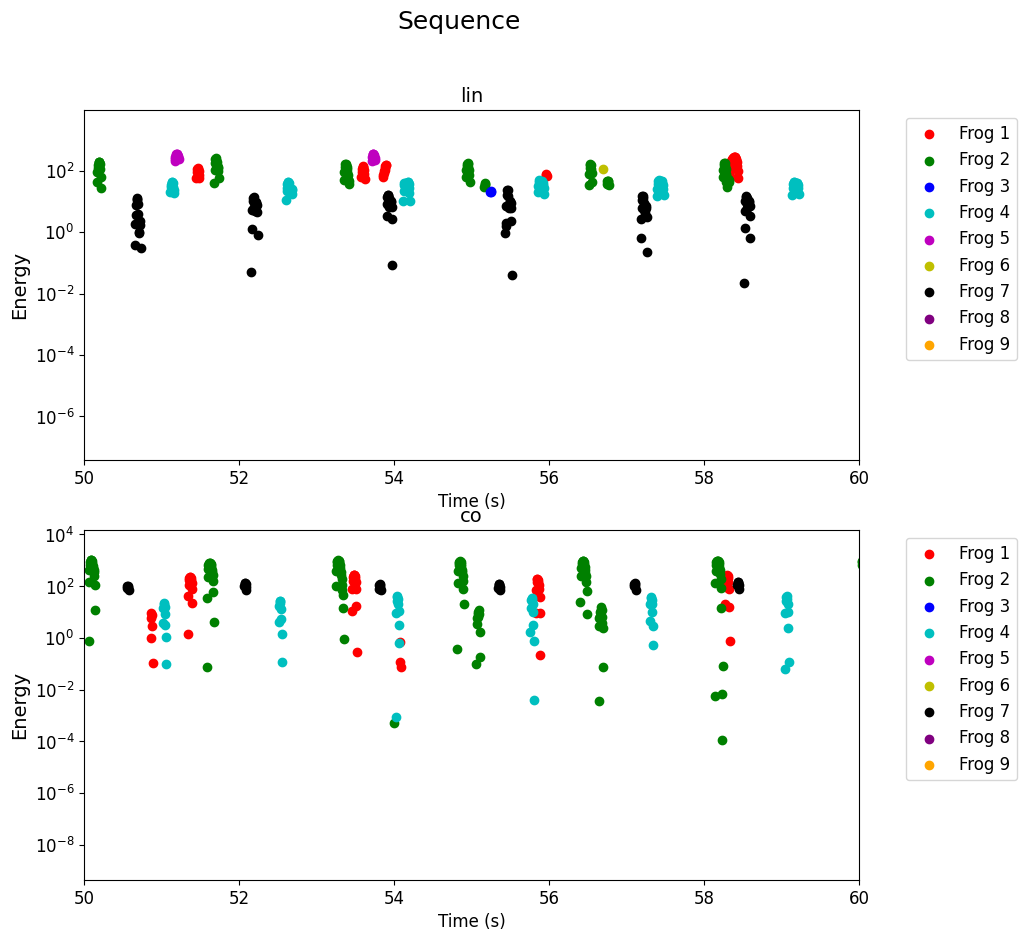
\includegraphics[width=\columnwidth]{Graphics/sequence.png}
    \caption{Fragmento de Secuencia de Cantos de los Colines en los archivos de \texttt{20231021\_190000}. Arriba la señales “LIN”, debajo los “CO”. Cada color representa una rana o micrófono diferente.}
    \label{fig:seq}
\end{figure}

En el intervalo analizado, las detecciones mantuvieron una 
periodicidad aproximada y una consistencia energética que 
parecen indicar la correcta detección y asignación de los cantos, 
condición 
imprescindible para avanzar hacia el estudio de las 
interacciones acústicas.

\subsection{Consistencia}
\label{sec:res_consistencia}

Para evaluar la consistencia del algoritmo, se realizaron diez 
ejecuciones independientes sobre el mismo conjunto de datos. En 
cada corrida se generaron nueve vectores (uno por micrófono-Colín), 
cada uno con los valores
de energía de los cantos asignados a ese micrófono, ubicados en los 
índices correspondientes a los instantes de tiempo en que fueron 
detectados los cantos. A fin de cuantificar la 
estabilidad de los resultados, se construyó una gran matriz de 
correlación cruzada entre todos los vectores provenientes de las 
diferentes ejecuciones.

La organización de la matriz siguió un orden bloque por bloque: 
primero se agruparon los vectores del micrófono “a” en cada una 
de las diez corridas, luego los del micrófono “b”, y así 
sucesivamente. De este modo, una alta correlación a lo largo de 
la diagonal principal indicaría que, para un mismo micrófono, 
las detecciones fueron reproducibles en cada ejecución.

La Figura~\ref{fig:correlation} presenta el mapa de calor de esa 
matriz. Se resaltaron en rojo las diez correlaciones más 
elevadas de cada fila. La evidente concentración de valores 
altos en la diagonal principal confirma que los vectores de 
detección correspondientes a un mismo micrófono exhibieron 
correlaciones significativamente mayores entre sí que con los 
vectores de otros canales. Este comportamiento empírico 
demuestra que el algoritmo produjo resultados coherentes y 
reproducibles.

\begin{figure}[ht]
    \centering
    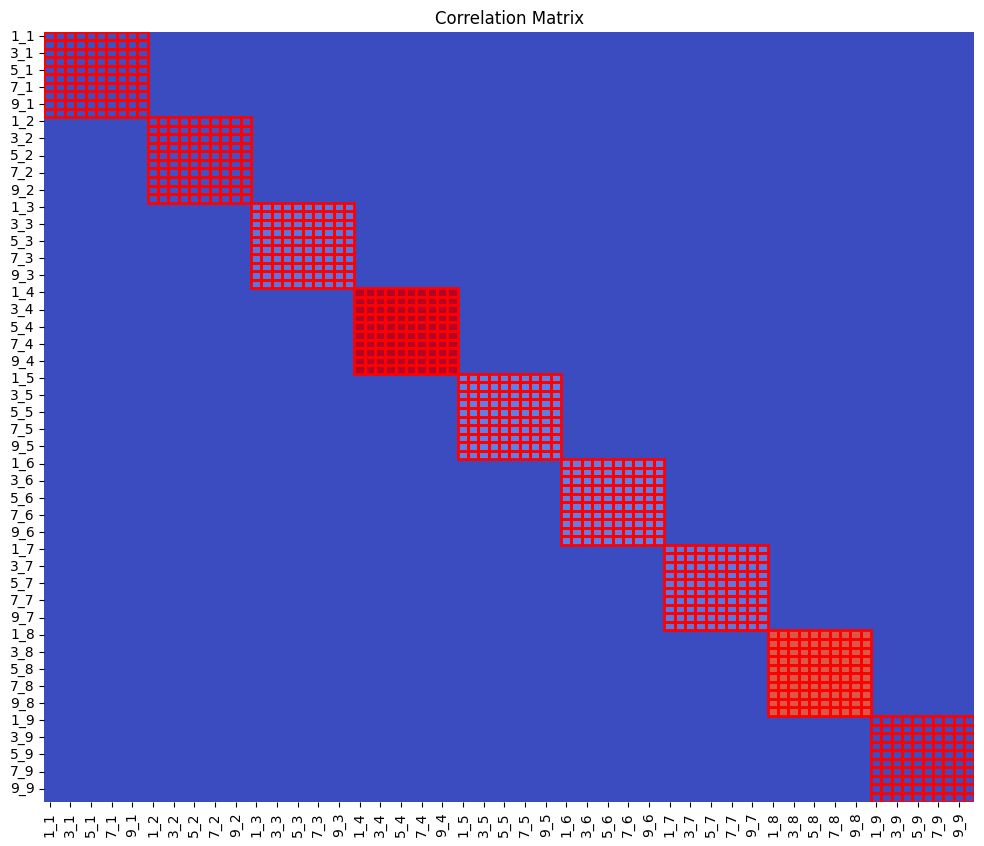
\includegraphics[width=0.7\linewidth]{Graphics/correlation_matrix.png}
    \caption{Matriz de correlación entre ejecuciones independientes del algoritmo sobre los datos de \texttt{20231021\_190000}. Los bloques diagonales de alta correlación (marcados en rojo) muestran la consistencia de las detecciones para cada micrófono.}
    \label{fig:correlation}
\end{figure}


\subsection{Comparación con detecciones manuales}

Para evaluar de forma cualitativa el desempeño de ambos 
algoritmos, se compararon sus detecciones con un etiquetado 
manual de cantos “CO” y “LIN” realizado sobre el conjunto de 
grabaciones de la sesión \texttt{20231021\_190000}. Dado que el 
etiquetado fue efectuado por personal no experto, esta comparación 
se abordó de manera visual y comparativa, sin aspirar a la 
rigurosidad de un protocolo validado por especialistas.  

En la Figura~\ref{fig:conf_mat_energies_cluster} se presenta la matriz de 
confusión del algoritmo basado en energías relativas (izq.) y 
la correspondiente al algoritmo de \textit{clustering} espectro-temporal (der.). 
Para esto se tomaron en cuenta solamente las grabaciones donde se detectaron
manualmente una gran cantidad de cantos.
Se consideró que un algoritmo había detectado correctamente un canto
cuando coincidía temporalmente (con tolerancia de 1 segundo) y en micrófono con los datos etiquetados.
Se observa 
que el método de \textit{clustering} obtuvo un mayor número de verdaderos 
positivos y menos falsos positivos que el de energías relativas. 
Ello se explica porque, cuando no todas las ranas estaban 
activas, el algoritmo de energías relativas tendía a asignar 
cantos a cada micrófono (incluso en aquellos donde no se encontraba cantando
ningún colín), elevando así sus falsos positivos y negativos. Por el 
contrario, el \textit{clustering} descartó los canales con actividad 
insuficiente, resultando más robusto en entornos de baja 
densidad acústica.  

\begin{figure}[ht]
  \centering
  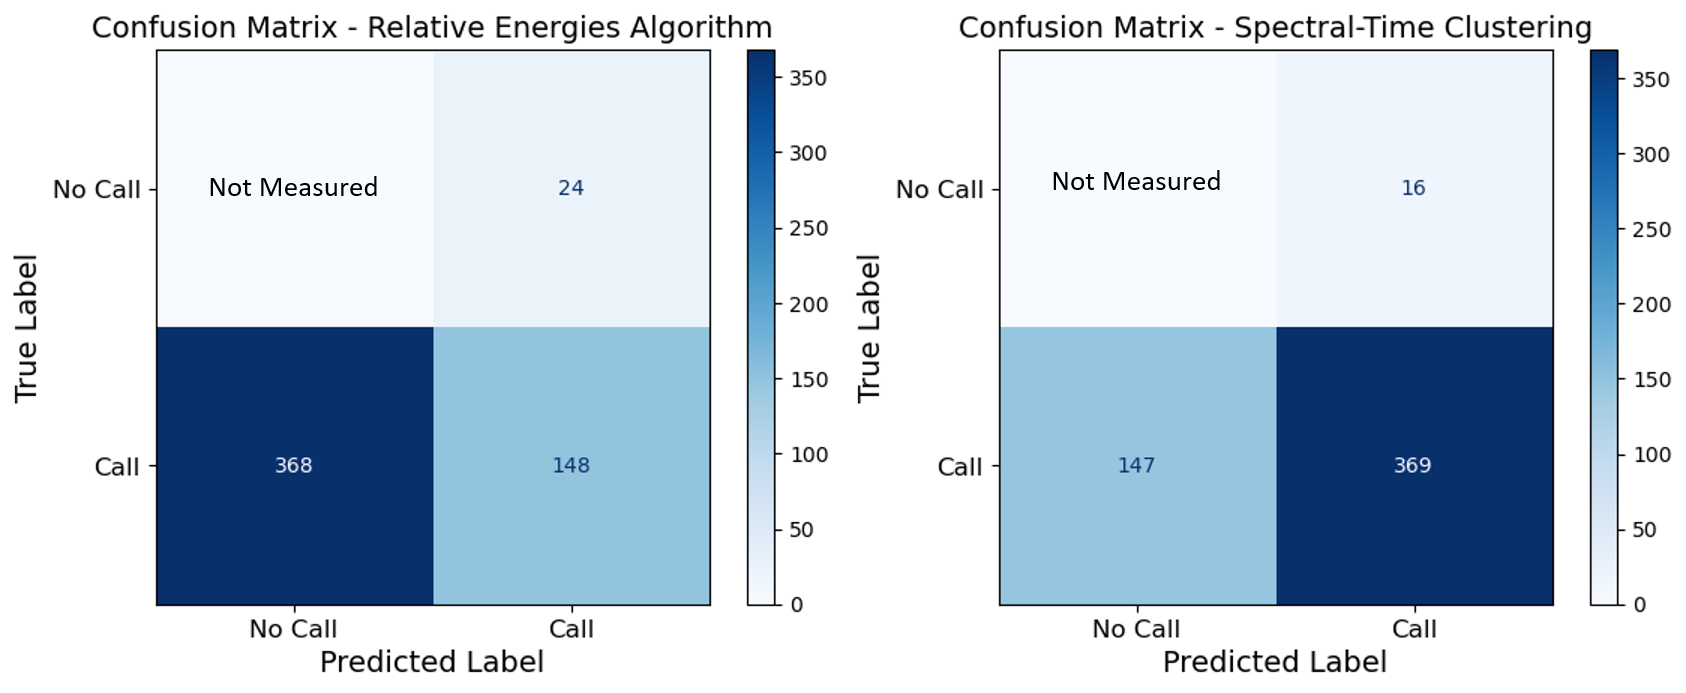
\includegraphics[width=\columnwidth]{Graphics/confusion_matrix_clustering_energies.png}
  \caption{Matriz de confusión del algoritmo de energías relativas vs.\ detecciones manuales (izq.). Matriz de confusión del algoritmo de \textit{clustering} espectro-temporal vs.\ detecciones manuales (der.). Solo se consideraron los cantos detectados en las grabaciones con mayor actividad.}
  \label{fig:conf_mat_energies_cluster}
\end{figure}



No se contabilizaron los verdaderos negativos (no canto) dado 
que dichos valores no forman parte de la salida de los 
algoritmos.  

Adicionalmente, se compararon los \(\Delta t\) (tiempo entre 
“CO” y su “LIN” correspondiente) obtenidos manualmente y por 
cada algoritmo. En el caso del método de energías, al ejecutarse
por separado en los “CO” y los “LIN”, algunos “CO” 
o “LIN” quedaron desemparejados y fueron filtrados mediante un 
umbral extraído del etiquetado manual. Tras este emparejamiento, 
el número de llamados considerados por el algoritmo de energías 
relativas bajó de 7 290 “LIN” y 9 863 “CO” a 5 467 pares, cifra 
cercana a los 5 964 pares hallados por \textit{clustering}.  

Los \textit{boxplots} y \textit{violinplots} de la Figura~\ref{fig:dt_box_violin} 
muestran que la distribución de \(|\Delta t|\) es muy similar 
entre el etiquetado manual, el algoritmo de energías y el de 
\textit{clustering}. Asimismo, los histogramas comparativos 
(Figura \ref{fig:histograms_deltas}) revelan 
alineamientos próximos de ambas técnicas con el patrón de 
referencia, a pesar de la posible imprecisión en los tags 
manuales.  

\begin{figure}[ht]
  \centering
  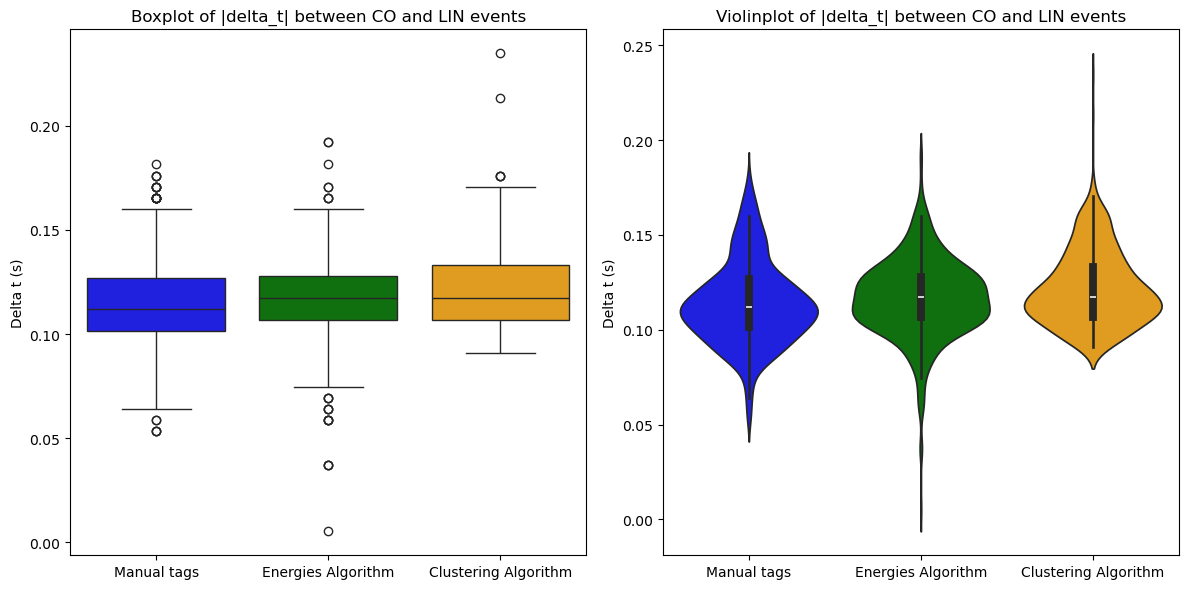
\includegraphics[width=\linewidth]{Graphics/boxplot_and_violin.png}
  \caption{\textit{Boxplot} y \textit{violinplot} de \(|\Delta t|\) entre “CO” y “LIN” para detecciones manuales, algoritmo de energías relativas y \textit{clustering}.}
  \label{fig:dt_box_violin}
\end{figure}

\begin{figure}[ht]
  \centering
  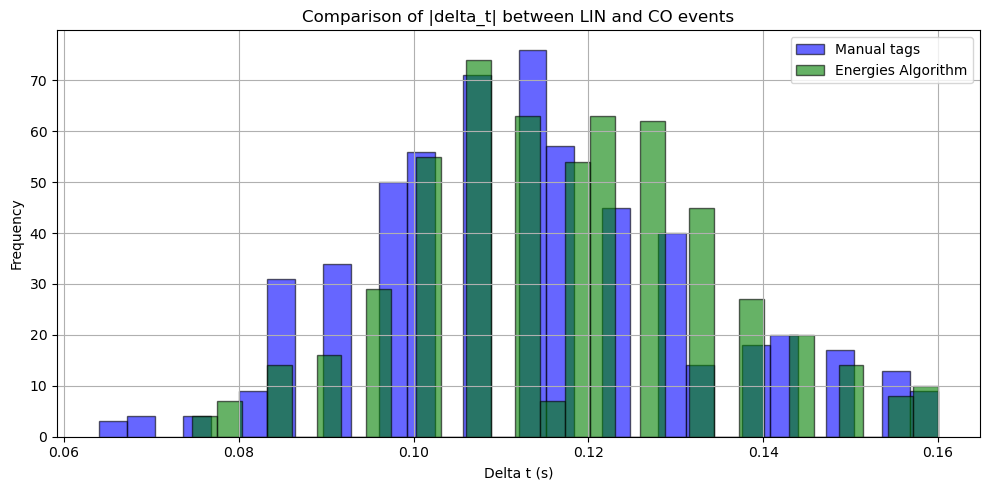
\includegraphics[width=0.48\linewidth]{Graphics/histogram_energies_tags.png}
  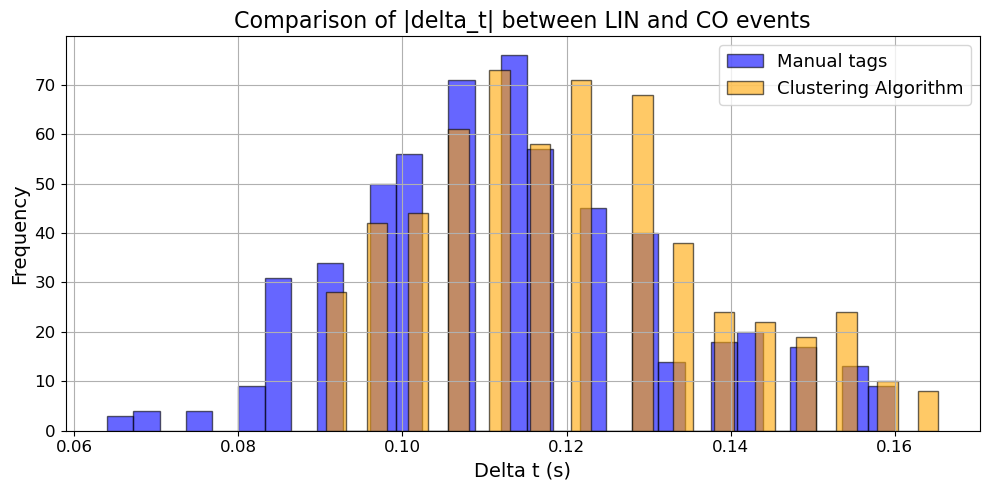
\includegraphics[width=0.48\linewidth]{Graphics/histogram_clustering_tags.png}
  \caption{Histogramas de \(\Delta t\): (izq.) manual vs.\ energías relativas; (der.) manual vs.\ \textit{clustering}. Los colores representan el origen de los datos (etiquetado manual, algoritmo de energías relativas o algoritmo de \textit{clustering}).}
  \label{fig:histograms_deltas}
\end{figure}

En conjunto, estos resultados sugieren que, comparándose con 
un etiquetado manual inexperto, el algoritmo basado en \textit{clustering}
muestra mejor rendimiento en cuanto a capturar la dinámica temporal del canto, 
pues ofrece mayor fiabilidad en escenarios de baja 
actividad. Para una validación estadística más rigurosa sería 
necesario un etiquetado experto que minimice el ruido de 
referencia.


% region Comparison
\section{Comparación entre algoritmos}
\label{sec:res_comparacion}


Con el objetivo de validar la robustez de los métodos propuestos 
para la detección y asignación de cantos, se compararon los 
resultados obtenidos mediante ambos algoritmos heurísticos 
presentados en el Capítulo anterior. 
La Figura~\ref{fig:alg_comparison} muestra un gráfico de 
dispersión que compara los tiempos de detección de cada canto 
individual en los archivos de \texttt{20231021\_190000}, con cada 
punto representando un canto detectado por ambos algoritmos y 
coloreado según el individuo correspondiente. La línea negra 
discontinua representa la identidad \( y = x \), indicando 
perfecta coincidencia entre ambos métodos. Por simplicidad,
el algoritmo descrito en la Sección~\ref{sec:alg_energia} (basado en energías relativas) 
se denominó \textbf{Algoritmo A} y el de la Sección~\ref{sec:alg_aglomerativo} (\emph{clustering} de espectro-tiempo),
\textbf{Algoritmo B}.

\begin{figure}[ht]
    \centering
    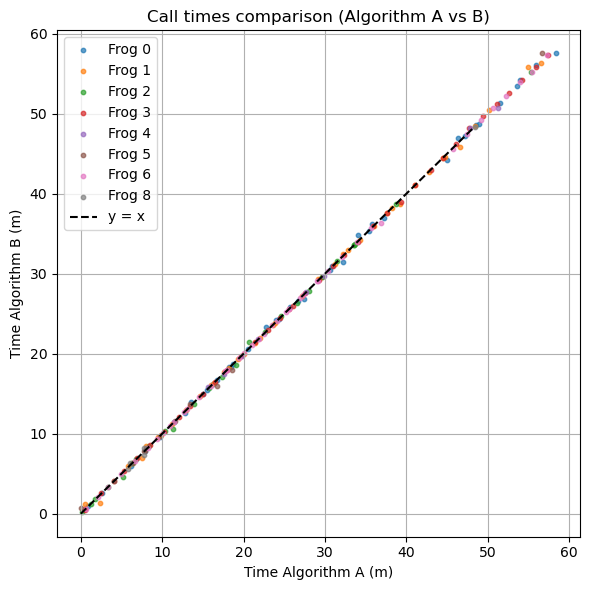
\includegraphics[width=0.7\linewidth]{Graphics/times_comparison.png}
    \caption{Comparación entre los tiempos de detección de cantos por los algoritmos A (energías relativas) y B (comportamiento de la especie) sobre los datos de \texttt{20231021\_190000}.}
    \label{fig:alg_comparison}
\end{figure}

Como puede observarse, la mayoría de los puntos se alinean con 
alta precisión sobre la recta de identidad, lo que indica un 
alto grado de concordancia entre ambos algoritmos en cuanto a 
los instantes de detección. Este resultado sugiere que, a pesar 
de basarse en supuestos distintos, ambos métodos producen 
secuencias temporales coherentes, lo cual refuerza la validez 
de los procedimientos desarrollados.

Para cuantificar con mayor precisión esta similitud, se realizó 
un ajuste lineal entre los tiempos de detección generados por 
ambos algoritmos para cada canal (o micrófono) por separado. Se 
calculó el coeficiente de determinación \( R^2 \), métrica 
comúnmente empleada para evaluar la calidad del ajuste de 
modelos lineales \cite{nagelkerke1991note}. Un valor cercano a 
\( R^2 = 1 \) reflejan una alta correlación.

La Tabla~\ref{tab:r2_results} resume los valores obtenidos de 
\( R^2 \) para los nueve canales analizados. En ocho de los 
casos se obtuvo un valor de \( R^2 = 1.00 \), indicando un 
solapamiento perfecto entre los resultados. Solo uno de los 
canales presentó un valor ligeramente inferior (\( R^2 = 0.99 \)), 
lo cual sigue siendo una indicación de coincidencia 
prácticamente total.

\begin{table}[ht]
    \centering
    \caption{Coeficientes de determinación \( R^2 \) del ajuste lineal entre algoritmos A y B por micrófono.}
    \label{tab:r2_results}
    \begin{tabular}{lc}
        \toprule
        \textbf{Micrófono} & \textbf{\( R^2 \)} \\
        \midrule
        \texttt{20231021\_190000a} & 1.00 \\
        \texttt{20231021\_190000b} & 1.00 \\
        \texttt{20231021\_190000c} & 1.00 \\
        \texttt{20231021\_190000d} & 1.00 \\
        \texttt{20231021\_190000e} & 0.999 \\
        \texttt{20231021\_190000f} & 1.00 \\
        \texttt{20231021\_190000g} & 1.00 \\
        \texttt{20231021\_190000h} & 1.00 \\
        \texttt{20231021\_190000i} & 1.00 \\
        \bottomrule
    \end{tabular}
\end{table}

Estos resultados corroboran que los algoritmos propuestos no 
solo son internamente consistentes, sino que ofrecen una 
detección altamente reproducible y concordante, 
independientemente del criterio heurístico considerado. 
Esta coincidencia refuerza la fiabilidad de las secuencias de 
canto extraídas, base fundamental para el análisis posterior de 
las interacciones acústicas en el sistema.




Adicionalmente, se analizaron las discrepancias en la detección 
de eventos “CO-LIN” entre ambos métodos. La 
Figura~\ref{fig:delta_hist} presenta el histograma comparativo 
de los \(\Delta t\) (diferencia temporal entre “CO” y “LIN”) 
detectados por el Algoritmo A y el Algoritmo B. 

\begin{figure}[ht]
    \centering
    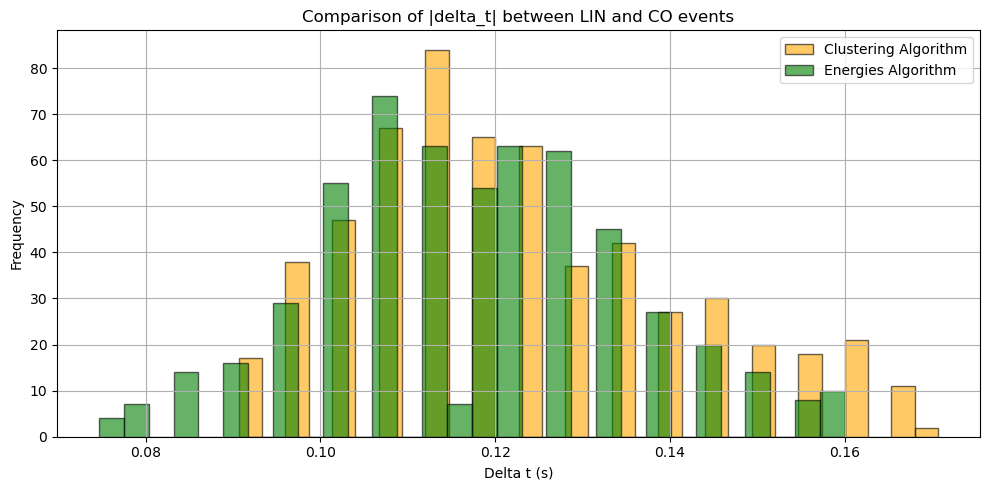
\includegraphics[width=\columnwidth]{Graphics/histogram_energies_clustering.png}
    \caption{Histogramas comparativos de \(\Delta t\) entre “CO” y “LIN” para el Algoritmo A (energías temporales) y el Algoritmo B (\textit{clustering} de espectro-tiempo).}
    \label{fig:delta_hist}
\end{figure}

Por último, se contabilizó cuántos cantos fueron detectados 
exclusivamente por cada algoritmo y cuántos coincidieron 
temporalmente (dentro de ±1 s) en el mismo micrófono. Los 
resultados fueron:
\begin{itemize}
  \item Solo detectados por Algoritmo A: 2429 cantos
  \item Solo detectados por Algoritmo B: 3000 cantos
  \item Detectados por ambos algoritmos: 3038 cantos
\end{itemize}

Estas cifras indican que el Algoritmo B (\textit{clustering}) 
identificó un mayor número de cantos no captados por el 
Algoritmo A, mientras que ambos detectaron conjuntamente la 
mayoría de eventos (3038). En particular, el Algoritmo A pasó 
por alto una parte significativa de cantos (2429 únicos de B 
frente a 3000 únicos de A), lo que refuerza la hipótesis de 
que su estrategia de 
energías relativas resulta menos sensible cuando no todos los 
individuos emiten simultáneamente. Por el contrario, el 
\textit{clustering} demostró una mayor cobertura de detección 
sin sacrificar la coincidencia temporal, confirmando su idoneidad 
en situaciones de actividad coral variable.

En conjunto, esta comparación demuestra que los dos algoritmos 
proporcionan resultados muy similares en cuanto a tiempo de 
detección (\(R^2\) casi unidad), pero difieren en sensibilidad: 
especialmente cuando no todos los Colines 
estaban activos simultáneamente, el método basado en \textit{clustering} 
(Algoritmo B) mostró mejor rendimiento general.



% region Ising
\section{Análisis de las interacciones inferidas \(\{J_{ij}\}\)}
\label{sec:res_interacciones}


La red de interacciones acústicas entre individuos fue inferida 
mediante el modelo de Ising descrito en el Capítulo anterior, 
utilizando configuraciones binarizadas de cantos. 
Este modelo permitió 
cuantificar la fuerza de acoplamiento entre pares de individuos, 
interpretada como una medida de influencia mutua en la emisión 
de vocalizaciones. 

En la Figura~\ref{fig:jij} se muestra la matriz simétrica 
\( J_{ij} \) obtenida para los datos de \texttt{20232110\_190000}. 
En ella, cada entrada 
representa la magnitud y dirección de la interacción inferida 
entre los individuos \( i \) y \( j \). Se observa una 
estructura dispersa, con varios acoplamientos claramente 
distintos de cero, lo que sugiere la existencia de vínculos 
acústicos no triviales entre ciertos miembros del coro. Las 
intensidades positivas indican una tendencia a la co-emisión 
simultánea, mientras que los valores negativos reflejan 
inhibición recíproca.

\begin{figure}[htbp]
    \centering
    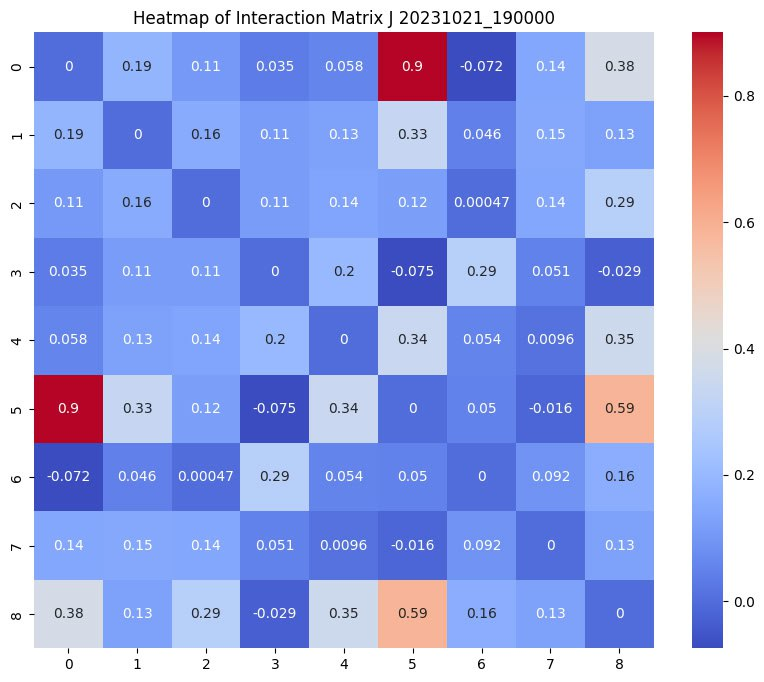
\includegraphics[width=0.7\linewidth]{Graphics/matrix_jij.jpg}
    \caption{Matriz de interacciones \( J_{ij} \) inferida para el \texttt{20231021\_190000}.}
    \label{fig:jij}
\end{figure}

Con el fin de facilitar la interpretación estructural de estas 
relaciones, se construyó un grafo no dirigido donde cada nodo 
representa a un individuo (o micrófono) y las aristas indican 
la existencia de interacciones significativas. En particular, 
se utilizó una línea continua para aquellas interacciones cuya 
magnitud supera el umbral de 0.5, y una línea discontinua para 
aquellas en el rango entre 0.3 y 0.5. Las conexiones cuyas 
magnituded resultaron inferiores a este último valor se consideraron 
insignificantes y fueron omitidas del grafo para mejorar la 
claridad visual. El resultado se presenta en la 
Figura~\ref{fig:graph}.

\begin{figure}[ht]
    \centering
    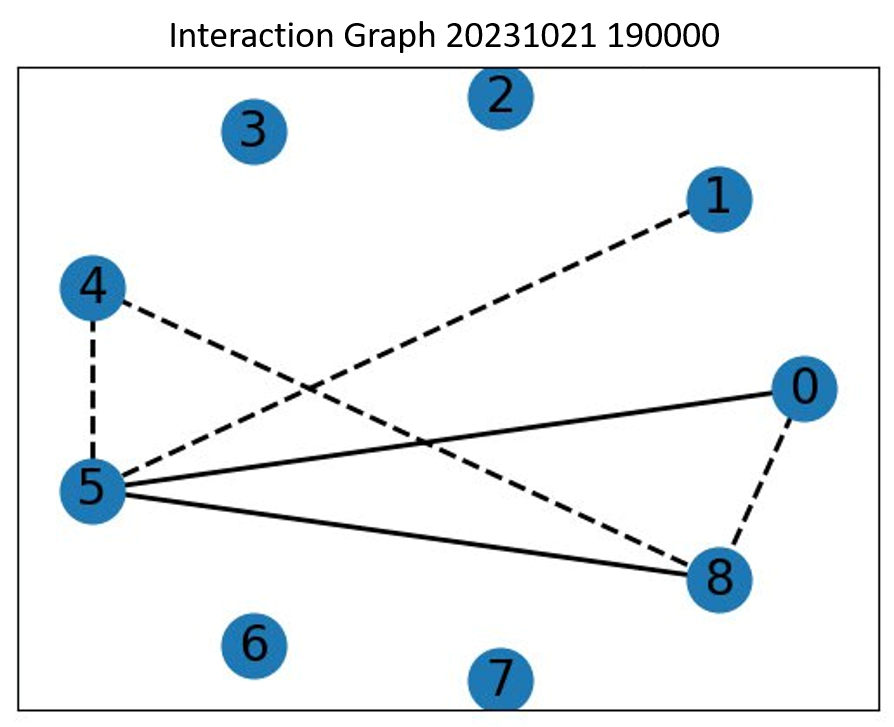
\includegraphics[width=0.7\linewidth]{Graphics/corr_graph.png}
    \caption{Grafo de interacciones correspondiente al \texttt{20231021\_190000}.}
    \label{fig:graph}
\end{figure}

Como análisis exploratorio adicional, se aplicó el mismo 
procedimiento de inferencia sobre tres intervalos horarios 
consecutivos de la misma noche (\texttt{20231021\_180000}, \texttt{20231021\_190000}, \texttt{20231021\_200000}). 
La Figura~\ref{fig:jij_evol} 
muestra la evolución de las matrices \( J_{ij} \) a lo largo 
de estas tres horas. Se observa que varias de las interacciones 
más fuertes (especialmente aquellas con valores superiores a 
0.5) se mantienen estables en el tiempo. Un ejemplo destacado es 
la interacción entre los individuos indexados como 0 y 5, que 
presenta una magnitud elevada y sostenida a lo largo del 
intervalo temporal analizado.

\begin{figure}[ht]
    \centering
    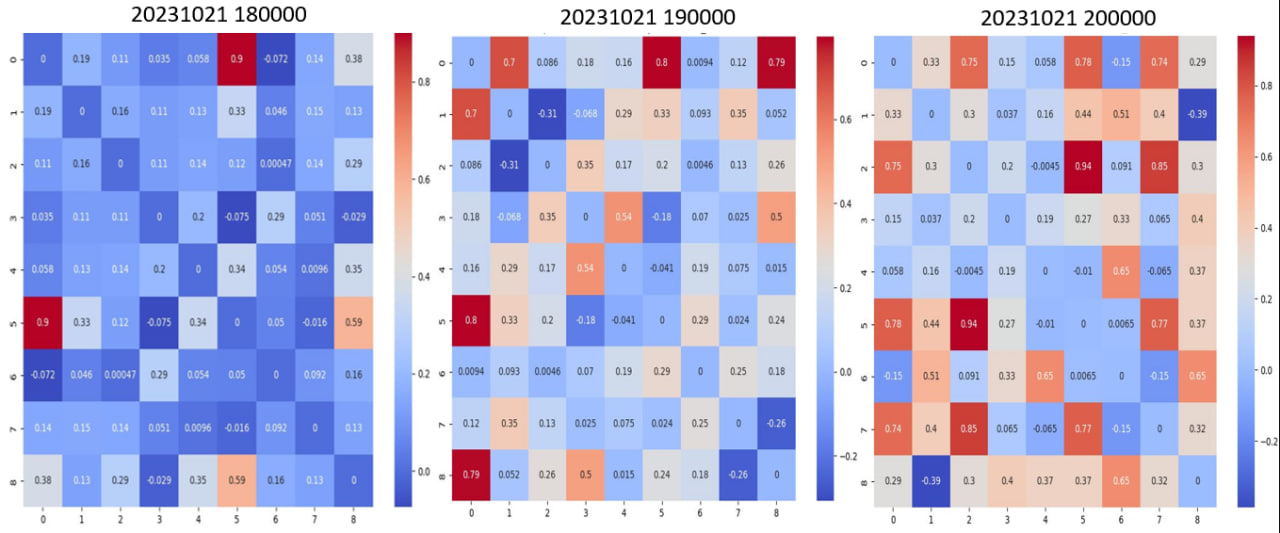
\includegraphics[width=\columnwidth]{Graphics/3_matrixs.jpg}
    \caption{Evolución de la matriz \( J_{ij} \) durante tres horas consecutivas (\texttt{20231021\_180000}, \texttt{20231021\_190000}, \texttt{20231021\_200000}).}
    \label{fig:jij_evol}
\end{figure}

Este patrón de persistencia fue también evidente en la 
representación gráfica de las redes inferidas, ilustradas en la 
Figura~\ref{fig:graph_evol}. La presencia continua de ciertas 
aristas a lo largo del tiempo sugiere la existencia de 
relaciones acústicas recurrentes y posiblemente funcionales 
entre algunos individuos. Dichos vínculos podrían reflejar 
mecanismos de coordinación o competencia territorial que 
merecen ser explorados en mayor profundidad en estudios futuros.

\begin{figure}[ht]
    \centering
    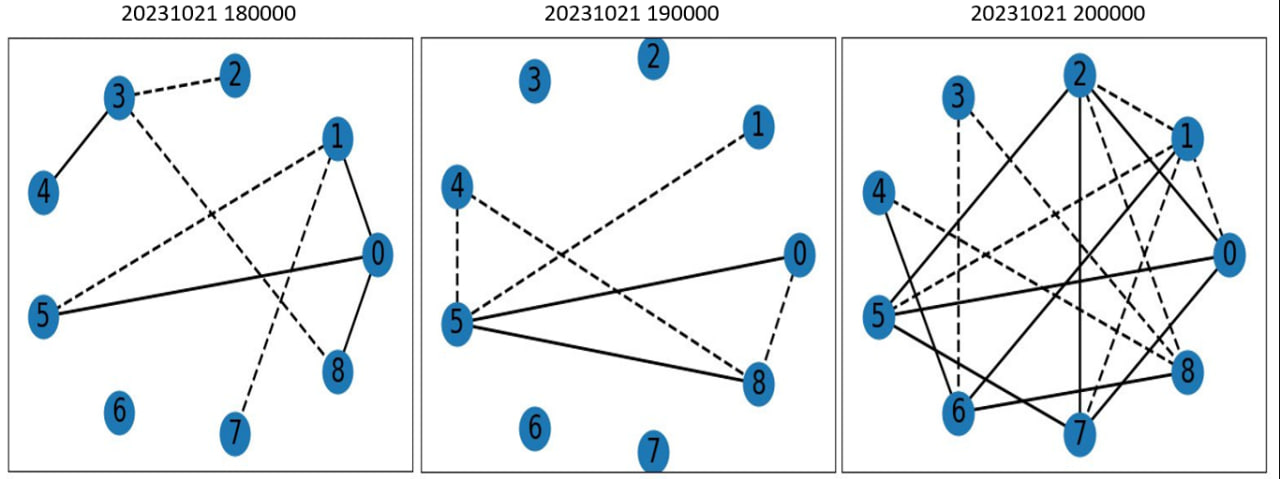
\includegraphics[width=\columnwidth]{Graphics/3_graphs.jpg}
    \caption{Evolución temporal de los grafos de interacciones inferidas para tres horas consecutivas (\texttt{20231021\_180000}, \texttt{20231021\_190000}, \texttt{20231021\_200000}).}
    \label{fig:graph_evol}
\end{figure}

Bajo el supuesto de que el modelo de Ising logra cantificar correctamente
las interacciones del sistema, estos hallazgos refuerzan la hipótesis de 
que los coros de 
\emph{E.\,eileenae} exhiben una estructura interna no aleatoria.


% region Idoneidad
\section{Análisis de idoneidad del modelo de Ising}
\label{sec:res_idoneidad}


Para evaluar la capacidad predictiva del modelo de Ising, se 
compararon sus estimaciones de la tasa de aparición de patrones 
de canto con las obtenidas bajo un modelo independiente en el 
que se asumen que cada Colín actúa sin influencia de los otros individuos 
\cite{schneidman2006weak}.

En la Figura~\ref{fig:ising_vs_indep} se presentan, en escala logarítmica, 
los patrones observados frente a los patrones predichos por 
ambos modelos para dos ventanas horarias distintas: \texttt{20231021\_190000}
y \texttt{20231021\_040000}. Cada punto corresponde a la frecuencia de un patrón 
particular de activación de espines (combinación de individuos 
cantando simultáneamente). La línea punteada \(y=x\) indica 
coincidencia perfecta entre observación y predicción.

\begin{figure}[ht]
    \centering
    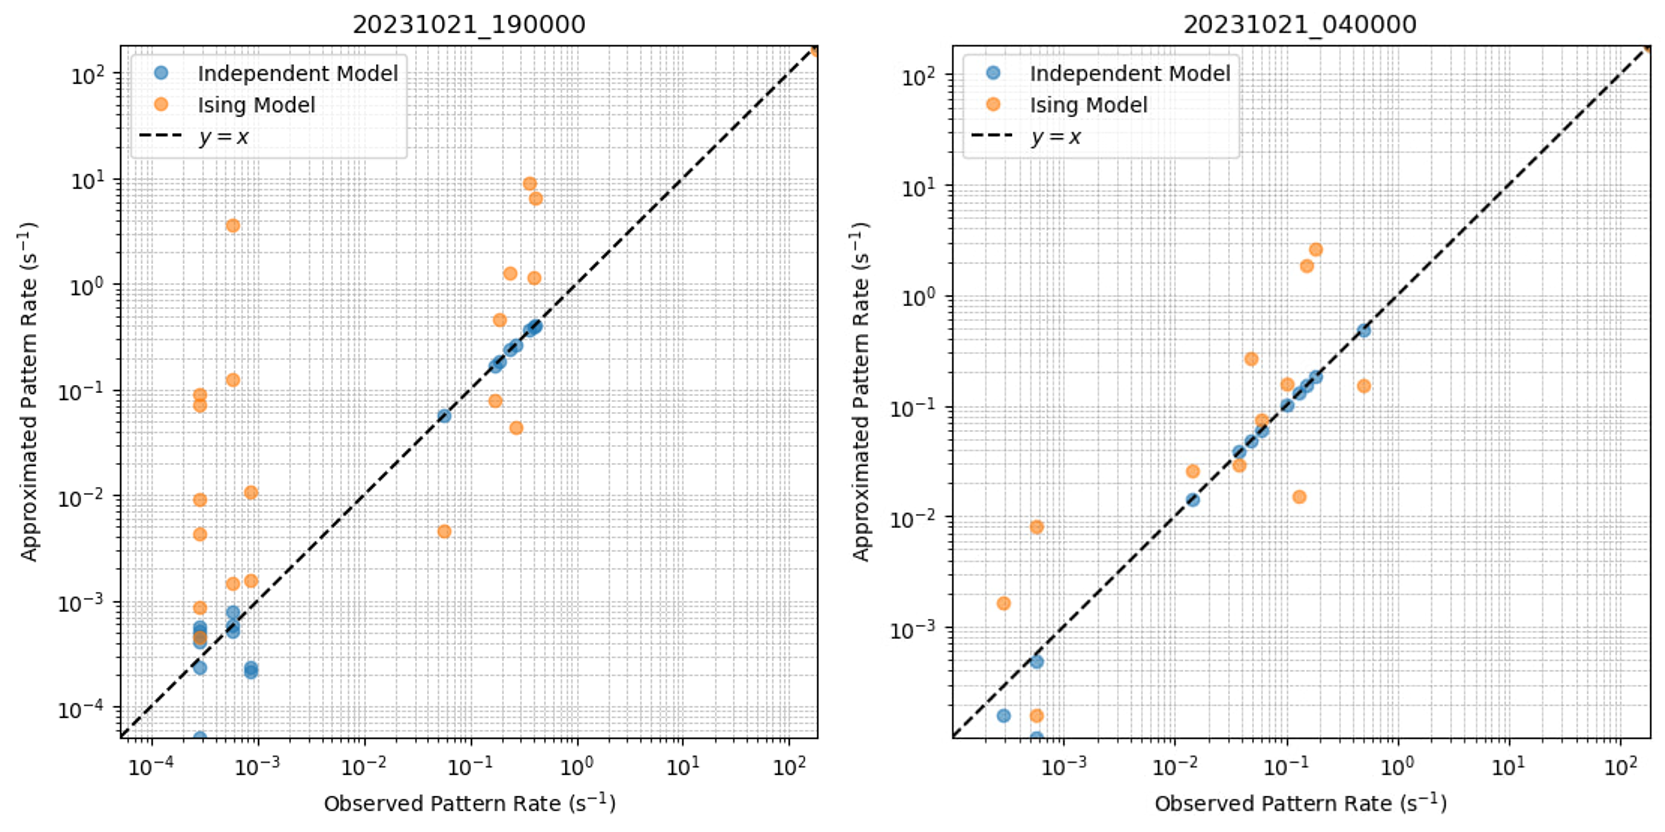
\includegraphics[width=\columnwidth]{Graphics/isingvsindependent.png}
    \caption{Tasa de aparición de patrones de canto observada versus predicha por el modelo independiente (azul) y el modelo de Ising (naranja) para las grabaciones de \texttt{20231021\_190000} (izq.) y \texttt{20231021\_040000} (der.).}
    \label{fig:ising_vs_indep}
\end{figure}

Contrariamente a lo esperado, el modelo independiente mostró una 
correspondencia más estrecha con las tasas observadas que el 
modelo de Ising, cuya predicción se desvió considerablemente en 
varios patrones de baja frecuencia. Este resultado sugiere al 
menos tres posibles interpretaciones: (1) las interacciones 
acústicas entre individuos podrían ser efectivamente débiles o 
nulas durante las ventanas analizadas, (2) el modelo de Ising, 
en su forma estacionaria y de segundo orden, podría no capturar 
adecuadamente la dinámica temporal o no lineal de los coros, o 
(3) la escasez de datos para patrones raros impide una estimación 
fiable de los parámetros de interacción. Esta última parece la más 
probable, dado que en la ejecución del descenso por gradiente se
escogió un \(\Delta t = 0\) para cuantificar las correlaciones entre
los espines (los Colines) a través de los estados del sistema. 
Esto puede estar arrojando resultados engañosos debido a que es 
mucho más probable un estado de -1 que de +1 (es mucho más tiempo en el que
los Colines no vocalizan que el tiempo en que lo hacen). 

En conjunto, estos hallazgos indican que, para el conjunto de 
grabaciones y la metodología empleada, el supuesto de 
independencia entre Colines resulta tan (o más) efectivo que el 
modelo de Ising para describir la distribución de patrones de 
canto. No obstante, la presencia de acoplamientos significativos 
observados en Sección~\ref{sec:res_interacciones} sugiere que 
podría ser necesaria una extensión del modelo (por ejemplo, 
incorporando términos de orden superior, efectos no 
estacionarios o dependencias temporales explícitas, así como explorar 
los valores del umbral de tiempo en el que se calculan las correlaciones) para 
capturar plenamente la complejidad del comportamiento grupal de 
\emph{E.\,eileenae}.




%\backmatter
%===================================================================================
% Chapter: Conclusiones
%===================================================================================
\chapter*{Conclusiones y Recomendaciones}\label{chapter:conclusions}
\addcontentsline{toc}{chapter}{Conclusiones y Recomendaciones}

%===================================================================================
% Chapter: Recomendaciones
%===================================================================================
\chapter*{Recomendaciones}\label{chapter:recomendations}
\addcontentsline{toc}{chapter}{Recomendaciones}


A partir de los hallazgos y limitaciones identificadas, se 
proponen las siguientes recomendaciones para futuras 
investigaciones:
\begin{itemize}
    \item \textbf{Mejorar la sincronización y validación}: 
    Incluir pulsos acústicos artificiales (tonos de referencia) 
    al inicio y final de cada grabación para facilitar la 
    alineación temporal. Paralelamente, colaborar con 
    bioacústicos expertos en \textit{E. eileenae} para generar 
    un \textit{ground truth} robusto mediante etiquetado manual 
    estandarizado, permitiendo métricas de evaluación más 
    rigurosas.
    
    \item \textbf{Ampliar la diversidad de datos}: Replicar el 
    estudio en múltiples temporadas reproductivas y localidades 
    geográficas, incorporando variables ambientales 
    (temperatura, humedad) para analizar su influencia en la 
    estructura de los coros. Esto enriquecería la generalidad de 
    los modelos propuestos.

    \item \textbf{Integrar información espacial}: Utilizar 
    micrófonos direccionales o arreglos de sensores para 
    triangular posiciones exactas de los individuos, combinando 
    datos acústicos con coordenadas georreferenciadas. Esta 
    información mejoraría la asignación de cantos y permitiría 
    modelar interacciones en función de distancias físicas.

    \item \textbf{Extender el modelo de interacciones}: Explorar modelos 
    alternativos como redes neuronales recurrentes o sistemas de 
    ecuaciones diferenciales acopladas, capaces de capturar 
    dependencias temporales y no lineales. Incorporar términos 
    de orden superior en el modelo de Ising, evaluar 
    formulaciones no estacionarias (fuera del equilibrio termodinámico)
    o inferir las correlaciones a través de un cálculo inteligente 
    del \(\Delta t\) de los estados de fase, son alternativas que
    podrían mejorar la 
    representación de la dinámica coral.

    \item \textbf{Analizar la regulación frecuencial como estrategia de segregación acústica}: 
    Profundizar en el estudio de las frecuencias características 
    de los cantos individuales de \textit{E. eileenae}, 
    evaluando si existen ajustes dinámicos que minimicen la 
    superposición espectral (multiplexación) dentro del coro.
    

\end{itemize}


Estas mejoras metodológicas, junto con la adopción de marcos 
teóricos más flexibles, potenciarían el estudio cuantitativo de 
sistemas bioacústicos complejos, tanto en anuros como en otras 
especies gregarias.
\renewcommand{\bibname}{Referencias Bibliográficas}
\nocite{*}
\bibliographystyle{plain}
\bibliography{build/Bibliography}
\include{BackMatter/Glossary}


\end{document}